\documentclass[12pt,letterpaper, onecolumn]{exam}
\usepackage{amsmath}
\usepackage{amssymb}
\usepackage{graphicx}
\usepackage{setspace}
\usepackage{nicefrac}
\setcounter{MaxMatrixCols}{20}
\usepackage[lmargin=71pt, tmargin=1.2in]{geometry}  %For centering solution box
\lhead{Optimal Estimation}
\rhead{Noah Miller}
\thispagestyle{empty}   %For removing header/footer from page 1

\begin{document}

\begingroup
\centering
\LARGE Optimal Estimation\\
\LARGE Homework 2 \\[0.5em]
\large \today\\[0.5em]
\large Noah Miller\par
\large 903949330\par
\large MECH 7710\par
\endgroup
\pointsdroppedatright   %Self-explanatory
\printanswers
\renewcommand{\solution}{\noindent\textbf{Ans:}\enspace}   %Replace "Ans:" with starting keyword in solution box


\begin{questions}
    \question{Two random variables $\mathbf{x}_1$ and $\mathbf{x}_2$ have a joint PDF that is uniform inside the circle (in the $\mathbf{x}_1-\mathbf{x}_2$ plane) with radius $2$, and zero outside the circle.}
    \begin{parts}
        \part{Find the math expression of the joint PDF function.}

        \solution{
            \begin{equation}
                \begin{split}
                    P_{x_1x_2} & =
                    \begin{cases}
                        \frac{1}{4\pi} & \text{if } \sqrt{x^2 + x_2^2} \leq 2 \\
                        0              & \text{if } \sqrt{x^2 + x_2^2} > 2    \\
                    \end{cases}
                \end{split}
            \end{equation}
        }

        \part{Find the conditional PDF $P_{x_2\vert x_1}(x_2\vert x_1 = 0.5)$?}

        \solution{
            We can find the conditional PDF by expanding equation \ref{eq:2}.
            \begin{equation}\label{eq:2}
                \begin{split}
                    P_{x_1 \vert x_2}(x_2\vert x_1 = 0.5) & = \frac{f_{x_1x_2}}{f_{x_1}}\\
                \end{split}
            \end{equation}
            Given that $x_1 = 0.5$ and our initial bounds, we can expand the denominator to be the PDF of $x_1$ or
            \begin{equation}
                \begin{split}
                    f_{x_1} & = \int^{-\sqrt{3.75}}_{-\sqrt{3.75}} \frac{1}{4\pi}dx_2\\
                    & = \frac{\sqrt{3.75}}{2\pi}
                \end{split}
            \end{equation}
            \begin{equation}
                \begin{split}
                    P_{x_1 \vert x_2}(x_2\vert x_1 = 0.5) & = \left(\frac{1}{4\pi}\right)\left(\frac{2\pi}{\sqrt{3.75}} \right)\\
                    & = \frac{1}{2\sqrt{3.75}}\\
                \end{split}
            \end{equation}
        }

        \part{Are the two random variables uncorrelated?}

        \solution{
            To find if the two random variables are uncorrelated, we start by calculating the covariance coefficient, $\rho_{12}$.
            \begin{equation}
                \begin{split}
                    \rho_{12} & = \frac{E[x_1,x_2] - \overline{x_1}\,\overline{x_2}}{\sigma_1 \sigma_2}\\
                \end{split}
            \end{equation}
            We can dissect this equation term by term to simplify it before solving.
            \begin{equation}
                \begin{split}
                    E[x_1,x_2] & = \int\int f_{x_1x_2}(x_1x_2)dx_1 dx_2\\
                    & = \int^{\sqrt{4-x_1^2}}_{-\sqrt{4-x_1^2}}\int^{\sqrt{4-x_2^2}}_{-\sqrt{4-x_2^2}} \frac{1}{4\pi}(x_1x_2)dx_1 dx_2\\
                    & = 0\\
                \end{split}
            \end{equation}
            Because the circle is centered about zero, we can assume the mean of $x_1$ and $x_2$ to be zero.
            \begin{equation}
                \begin{split}
                    \overline{x_1} & = 0\\
                    \overline{x_2} & = 0\\
                \end{split}
            \end{equation}
            With the numerator of the covariance coefficient equally 0, we can effectively say that $\rho_{12} = 0$. Because of this the off-diagonal terms of the covariance matrix are 0, proving that the two random variables are uncorrelated.
        }

        \part{Are the two random variables statistically independent?

            \textit{Hint: find} $p_{x_1}(x_1)$ and $p_{x_2}(x_2)$ and check if $p_{x_1x_2}(x_1,x_2) = p_{x_1}(x_1)p_{x_2}(x_2)$
        }

        \solution{
            No. The two random variables ($x_1$,$x_2$) are not statistically independent. We can prove this using the property from our notes: \[f_{x_1 x_2} = f_{x_1} f_{x_2} \]
            Using our previous method from part \textbf{b} and substituting our integration limits from part \textbf{c} gives us:
            \begin{equation}
                \begin{split}
                    f_{x_1} & = \int^{\sqrt{4-x^2_1}}_{-\sqrt{4-x^2_1}}\frac{1}{4\pi}dx_1\\
                    & = \frac{x_2}{4\pi}\bigg\vert^{\sqrt{4-x^2_1}}_{-\sqrt{4-x^2_1}}\\
                    & = \frac{\sqrt{4-x^2_1}}{4\pi} + \frac{\sqrt{4-x^2_1}}{4\pi}\\
                    f_{x_1} & = \frac{\sqrt{4-x^2_1}}{2\pi} \\
                \end{split}
            \end{equation}
            The PDF for $f_{x_2}$ is very similar, only differing by changing $x_1$ to $x_2$.
            \begin{equation}
                \begin{split}
                    f_{x_2} & = \frac{\sqrt{4-x^2_2}}{2\pi} \\
                \end{split}
            \end{equation}
        }
    \end{parts}
    \clearpage
    \question{The stationary process $\mathbf{x}(t)$ has an autocorrelation function of the form: \[R_x(\tau) = \sigma^2 e^{-\beta \vert \tau \vert} \]
        Another process $\mathbf{y}(t)$ is related to $\mathbf{x}(t)$ by the deterministic equation: \[y(t) = ax(t) + b \] where the constants $\mathbf{a}$ and $\mathbf{b}$ are known.}
    \begin{parts}
        \part{What is the auto-correlation function for $\mathbf{y}(t)$}

        \solution{We know the general form of the auto-correlation function to be
            \[R(t,\;t + \tau) = E\left[y(t)y(t + \tau)\right], \]
            and by substituting our given function of $y(t)$, we find our general form to reflect:
            \begin{equation}
                \begin{split}
                    R(t,\;t+\tau) & = E\left[(ax(t) + b)(ax(t + \tau) + b)\right]\\
                    & = E\left[(a^2x(t)x(t + \tau) + bax(t + \tau) + bax(t) + b^2)\right]\\
                    & = E\left[(a^2x(t)x(t + \tau) + bax(t + \tau) + bax(t) + b^2)\right]\\
                    & = a^2 E\left[x(t)x(t + \tau)\right] + baE\left[x(t + \tau)\right] + baE\left[x(t)\right] + E\left[b^2\right]\\
                    & = a^2 \sigma^2 e^{-\beta \vert \tau \vert} + 2ba\overline{x}\\
                \end{split}
            \end{equation}}

        \part{What is the cross-correlation function $R_{xy}(\tau) = E\left[x(t)y(t + \tau) \right]$?}

        \solution{Similiar to how we started part a, we substitute our given function for $y(t)$ and solve.
            \begin{equation}
                \begin{split}
                    R_{xy}(\tau) & = E\left[x(t)y(t + \tau) \right]\\
                    & = E\left[x(t)\left(ax(t + \tau) + b\right)\right]\\
                    & = E\left[x(t)ax(t + \tau) + bx(t)\right]\\
                    & = aE\left[x(t)x(t + \tau)\right] + bE\left[x(t)\right]\\
                    & = a \sigma^2 e^{-\beta \vert \tau \vert} + b \overline{x}\\
                \end{split}
            \end{equation}}
    \end{parts}
    \clearpage
    \question{Use least squares to indentify a gyroscopes scale factor (a) and bias(b). Simulate the gyroscope using: \[g(k) = ar(k) + b + n(k) \] \[n \sim N\left(0,0.3 \left[\frac{rads}{s}\right]\right) \] \[r(t) = 100sin(\omega t) \]}
    \begin{parts}
        \part{Perform the least squares with 10 samples (make sure to pick $\omega$ so that you get one full cycle in 10 samples).}

        \solution{
            To make sure my least squares process is correct, displayed below are figures of the noise (figure 1), the true rotation (figure 2) and the gyroscope measurement with the added scale factor and bias (figure 3). Setting my $a$ and $b$  to $5$ and $0.5$, repectively, produced an estimated value of those parameters as $4.9967$ and $0.6872$.

            \begin{figure}[!h]
                \centering
                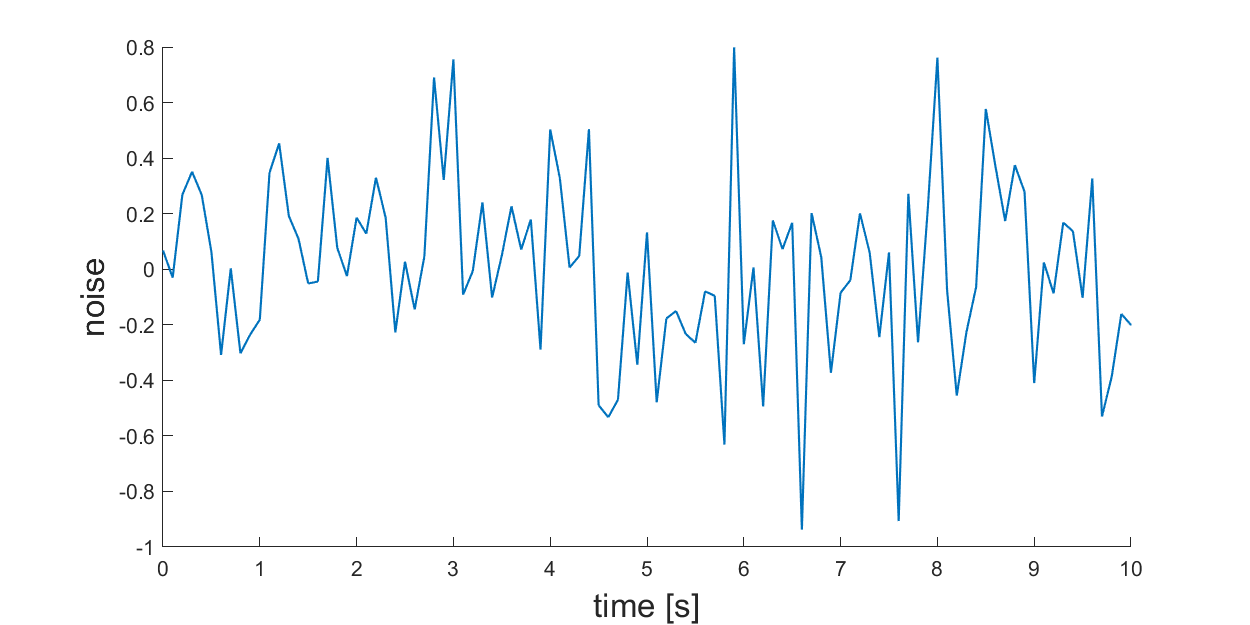
\includegraphics[width=.65\linewidth]{Q3a_n.png}
                \caption{10 samples of simulated noise being added to the system.}
                \label{fig:1}
            \end{figure}

            \begin{figure}[!h]
                \centering
                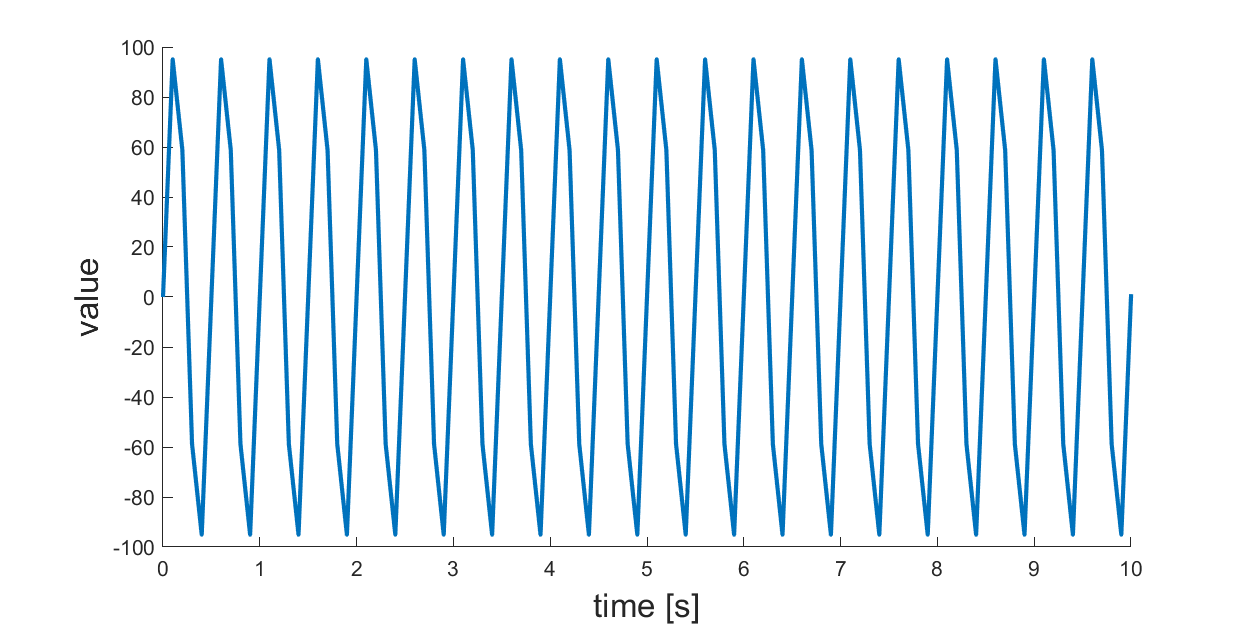
\includegraphics[width=.65\linewidth]{Q3a_r.png}
                \caption{10 samples of system rotation with \underline{no} noise added.}
                \label{fig:2}
            \end{figure}

            \begin{figure}[!h]
                \centering
                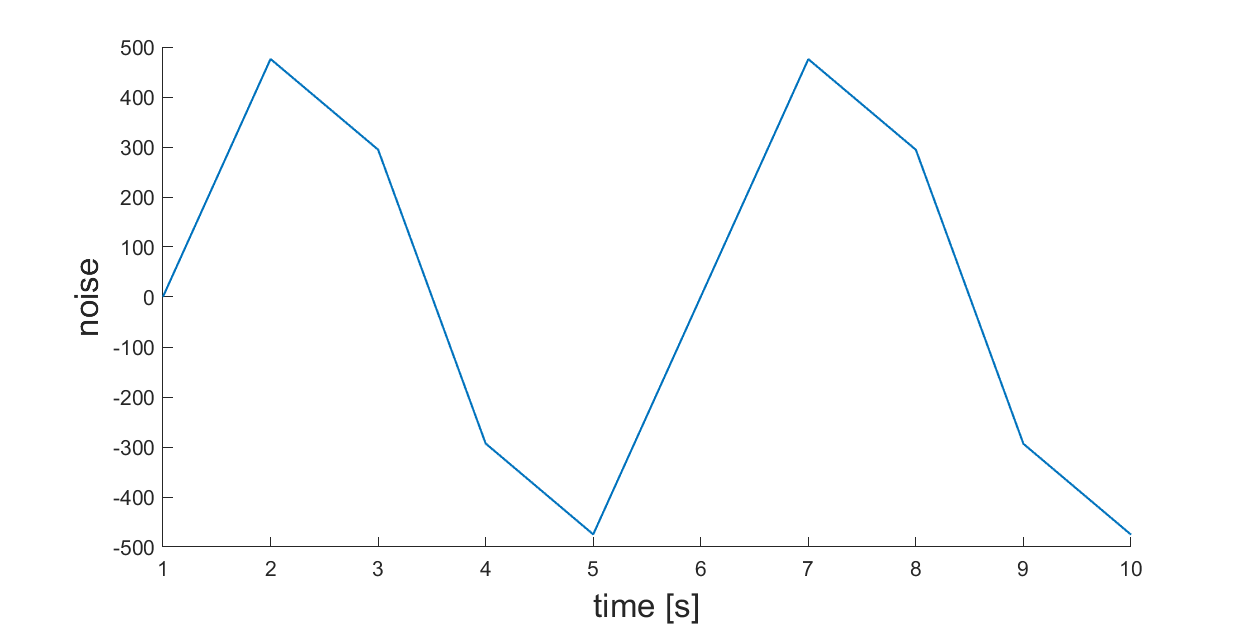
\includegraphics[width=.7\linewidth]{Q3a_g.png}
                \caption{Simulated raw measurements from gyroscope.}
                \label{fig:3}
            \end{figure}
        }
        \part{Repeat part (a) 1000 times and calculate the mean and standard deviation of the estimate errors (this is known as a Monte Carlo Simulation). Compare the results to the theoretically expected mean and standard deviation.}

        \solution{
            Running the same 10 samples over 1000 times produced the following results (figure \ref{fig:4}). Through the 1000-run monte-carlo simulation, we get a mean of $4.999$ for a value of $a$ and a mean of $0.4983$ for $b$. This pretty close to our expected mean $5$ and $0.5$.
            Furthermore, we get a standard deviation of $0.0013304$ for a value of $a$ and a standard deviation of $0.093126$ for $b$. This pretty close to our expected standard deviation $0.0018$ and $0.09$.
            \begin{figure}[!h]
                \centering
                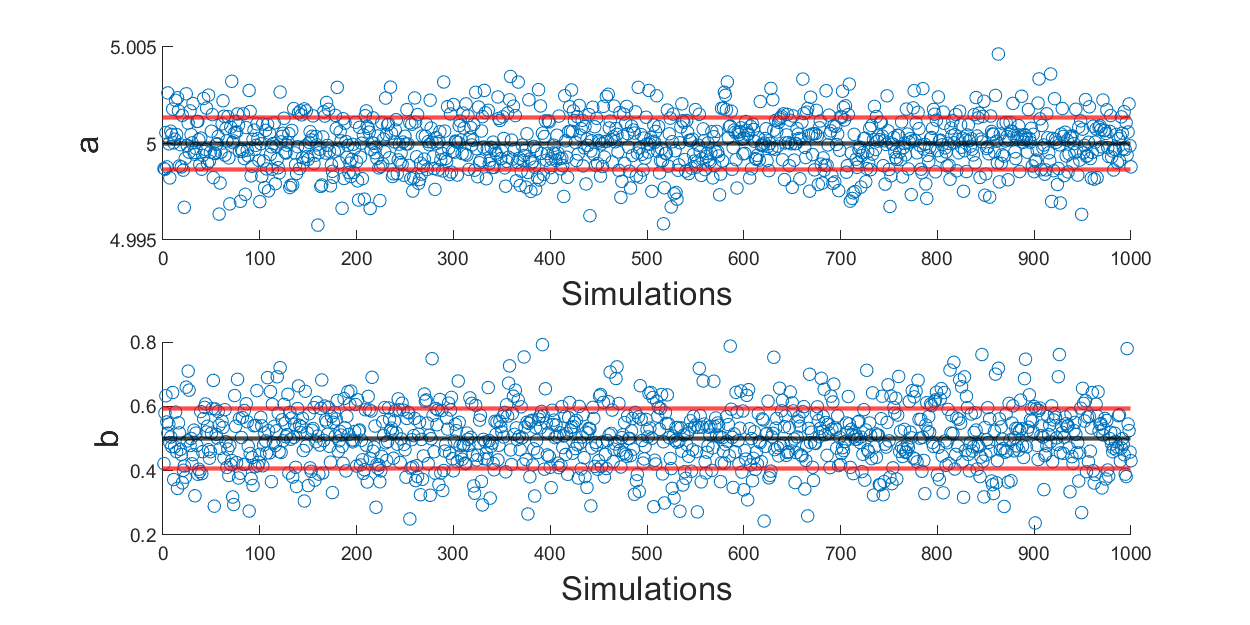
\includegraphics[width=\linewidth]{Q3a_1000.png}
                \caption{1000-run Monte-Carlo simulation using least squares.}
                \label{fig:4}
            \end{figure}
        }
        \clearpage
        \part{Repeat part (a) and (b) using 1000 samples. What does the theoretical and Monte Carlo standard deviation of the estimated errors approach?}

        \solution{
            Doing 1000 samples per simulation allows to approach the expected mean and standard deviation more closely than doing 10 samples per simulation.
            \begin{figure}[!h]
                \centering
                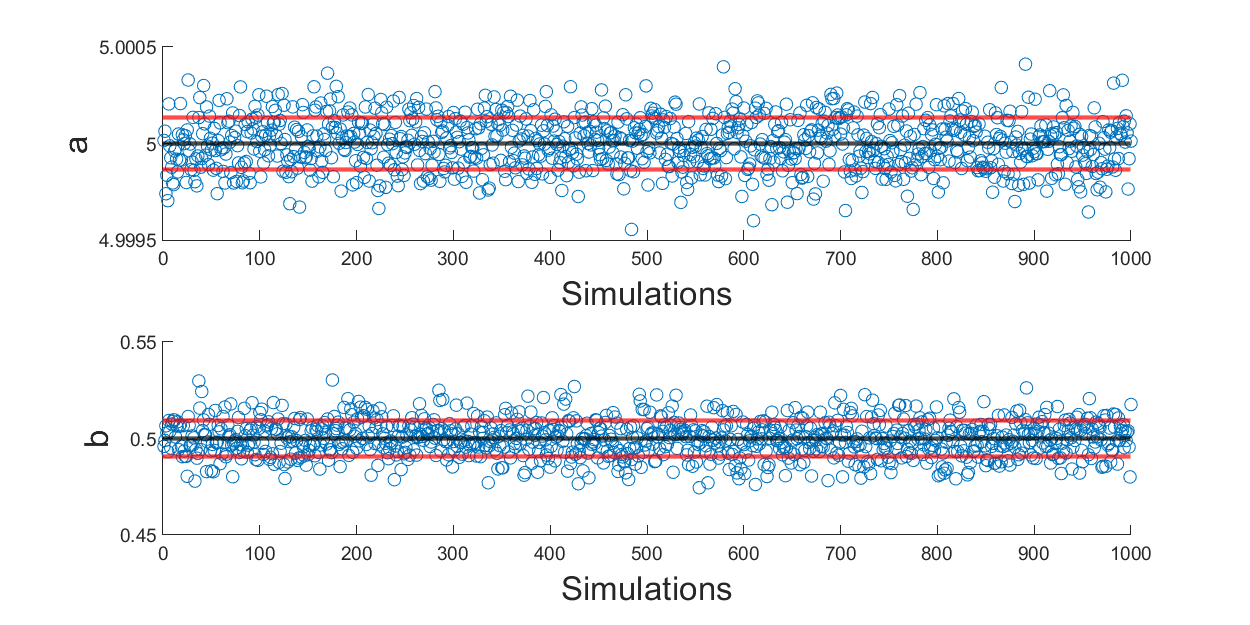
\includegraphics[width=\linewidth]{Q3c_10000.png}
            \end{figure}
        }

        \part{Set up the problem to run as a recursive least squares and plot the coefficients and theoretical standard deviation of the estimate error and the actual estimate error as a function of time.}

        \solution{
            Using recursive least squares gives an accurate estimation of the coefficients, seen in the figure below. The mean and standard deviation values for the recursive least squares method deviates a tiny bit at the beginning, but is spot on to the exact values as time progresses.
            \begin{figure}[!h]
                \centering
                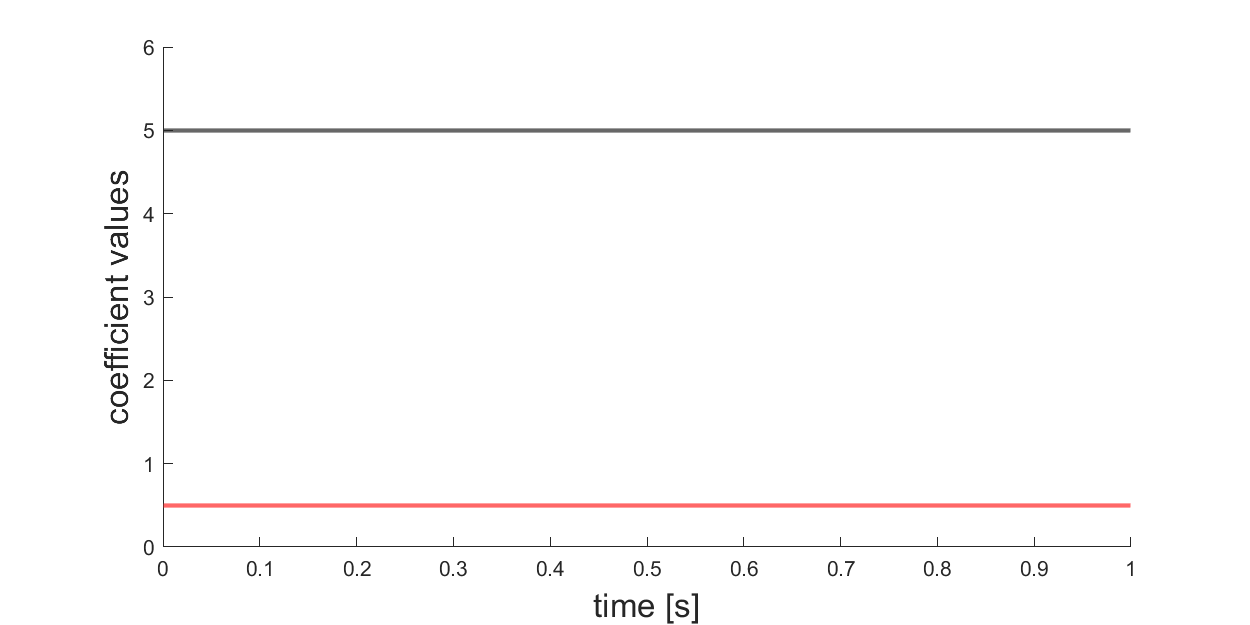
\includegraphics[width=0.75\linewidth]{Q3d.png}
                \caption{Coefficient estimation using recursive least squares.}
                \label{fig:5}
            \end{figure}
        }
        \clearpage
    \end{parts}
    \question{\textbf{Least Squares for System (I.D.)}
        Simulate the following discrete system with normal random input and output noise \[G(z) = \frac{0.25(z - 0.8)}{z^2 - 1.90z + 0.95} \]
        Paste the following sample MATLAB code to do this
        \begin{equation}
            \begin{split}
                >> & numd  = 0.25\cdot[\:1 \quad -0.8\:]\\
                >> & dend  = [\:1 \quad -1.9\quad 0.95 \:]\\
                >> & u  = randn(1000,1)\\
                >> & y  = dlsim(numd,dend,u)\\
                >> & sigma  = 0.01\\
                >> & Y = y + sigma\cdot randn(1000,1)\\
            \end{split}
        \end{equation}
    }
    \begin{parts}
        \part{Develop the $\mathbf{H}$ matrix for the least squares solution.}

        \solution{%
            We can find the measurement matrix, $\mathbf{H}$, by converting our system to discrete and then transforming the equation to matrix form (Equation \eqref{eq:13}).
            \begin{equation}
                \begin{split}
                    G(z) & = \frac{0.25(z - 0.8)}{z^2 - 1.90z + 0.95}\\
                    \frac{Y(z)}{U(z)} & = \frac{0.25(z - 0.8)}{z^2 - 1.90z + 0.95}\cdot \frac{z^{-2}}{z^{-2}}\\
                    Y(z)(1 - 1.90z^{-1} + 0.95z^{-2}) & = U(z)(0.25z^{-1} - 0.2z^{-2})\\
                    Y(n) - 1.9\,Y(n-1) + 0.95\,Y(n-2) & = 0.25\,U(n-1) - 0.2\,U(n-2)\\
                \end{split}
                \label{eq:13}
            \end{equation}
            If we isolate $Y(n)$, the system can be put into matrix form by having the input and output terms as the body of the measurement matrix and the coefficients as the state matrix.
            \begin{equation}
                Y(n) = 0.25\,U(n-1) - 0.2\,U(n-2) + 1.9\,Y(n-1) - 0.95\,Y(n-2)
            \end{equation}
            \begin{equation}
                \begin{split}
                    \mathbf{Y} & = \mathbf{Hx}\\
                    \mathbf{Y} & =
                    \begin{bmatrix}
                        y_0    \\
                        y_1    \\
                        y_2    \\
                        \vdots \\
                        y_n    \\
                    \end{bmatrix}\\
                    \mathbf{H} & =
                    \begin{bmatrix}
                        u_{n-1} & u_{n-2} & y_{n-1} & y_{n-2} \\
                        u_{0}   & u_{n-1} & y_{0}   & y_{n-1} \\
                        u_{1}   & u_{0}   & y_{1}   & y_{0}   \\
                        \vdots  & \vdots  & \vdots  & \vdots  \\
                        u_{n-1} & u_{n-2} & y_{n-1} & y_{n-2} \\
                    \end{bmatrix}\\
                \end{split}
                \label{eq:15}
            \end{equation}
            Because we are trying to estimate the state of the system, $\mathbf{x}$ will be in variable form and not the coefficients.
            \begin{equation}
                \begin{split}
                    \mathbf{x} & =
                    \begin{bmatrix}
                        x_1 \\
                        x_2 \\
                        x_3 \\
                        x_4 \\
                    \end{bmatrix}
                \end{split}
                \label{eq:16}
            \end{equation}
        }

        \part{Use the least squares to estimate the coefficients of the above Transfer Function.}
        \begin{subparts}
            \subpart{How good is the fit?}

            \solution{%
                We can setup least squres for the system simmiliarly to problem 3.
                \begin{equation}
                    \begin{split}
                        \mathbf{x}& = \left(\mathbf{H}^T\mathbf{H}\right)^{-1}\mathbf{H}^T \mathbf{Y}\\
                        \begin{bmatrix}
                            x_1 \\
                            x_2 \\
                            x_3 \\
                            x_4 \\
                        \end{bmatrix} & = \left(
                        \begin{bmatrix}
                            u_{n-1} & u_{n-2} & y_{n-1} & y_{n-2} \\
                            u_{0}   & u_{n-1} & y_{0}   & y_{n-1} \\
                            u_{1}   & u_{0}   & y_{1}   & y_{0}   \\
                            \vdots  & \vdots  & \vdots  & \vdots  \\
                            u_{n-1} & u_{n-2} & y_{n-1} & y_{n-2} \\
                        \end{bmatrix}^T
                        \begin{bmatrix}
                            u_{n-1} & u_{n-2} & y_{n-1} & y_{n-2} \\
                            u_{0}   & u_{n-1} & y_{0}   & y_{n-1} \\
                            u_{1}   & u_{0}   & y_{1}   & y_{0}   \\
                            \vdots  & \vdots  & \vdots  & \vdots  \\
                            u_{n-1} & u_{n-2} & y_{n-1} & y_{n-2} \\
                        \end{bmatrix}\right)^{-1}\\
                        \cdot &\begin{bmatrix}
                            u_{n-1} & u_{n-2} & y_{n-1} & y_{n-2} \\
                            u_{0}   & u_{n-1} & y_{0}   & y_{n-1} \\
                            u_{1}   & u_{0}   & y_{1}   & y_{0}   \\
                            \vdots  & \vdots  & \vdots  & \vdots  \\
                            u_{n-1} & u_{n-2} & y_{n-1} & y_{n-2} \\
                        \end{bmatrix}^T \begin{bmatrix}
                            y_0    \\
                            y_1    \\
                            y_2    \\
                            \vdots \\
                            y_n    \\
                        \end{bmatrix}\\
                    \end{split}
                    \label{}
                \end{equation}
                \begin{equation}
                    \begin{bmatrix}
                        x_1 \\
                        x_2 \\
                        x_3 \\
                        x_4 \\
                    \end{bmatrix}  =
                    \begin{bmatrix}
                        0.24948 \\
                        0.19818 \\
                        1.8931  \\
                        0.94336 \\
                    \end{bmatrix}
                \end{equation}
            }
            \clearpage
            \subpart{Plot the bode response of the I.D. TF and simulated TF on the same plot.}

            \solution{%
                \begin{figure}[!h]
                    \centering
                    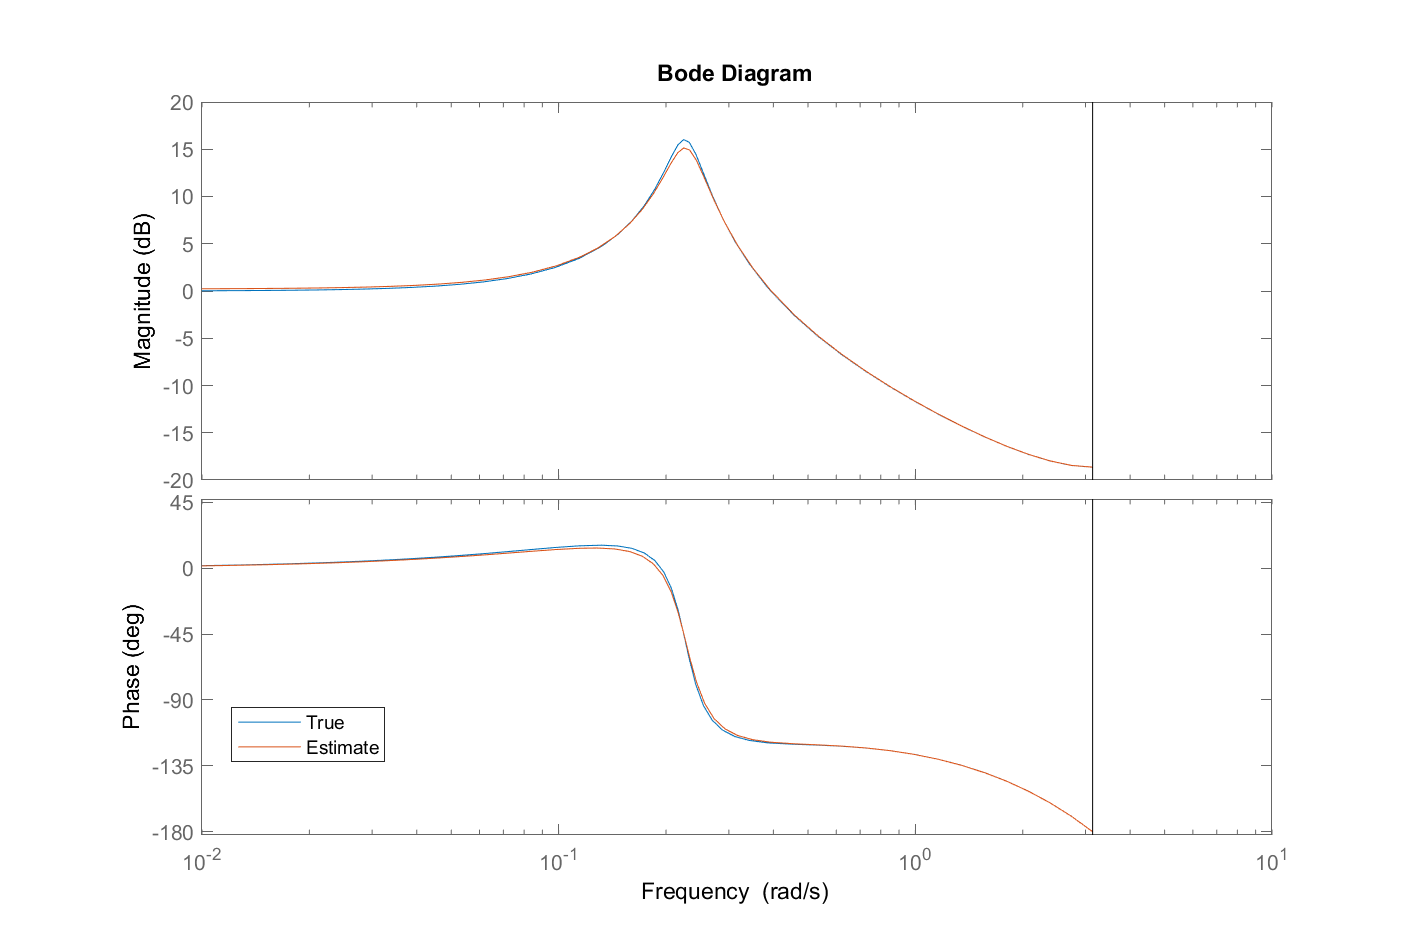
\includegraphics[width=\linewidth]{bode_4b.png}
                    \caption{Bode comparison of estimated and true states from Equation \eqref{eq:15}}
                    \label{fig:6}
                \end{figure}
            }
            \clearpage
            \subpart{How much relative noise has been added (SNR - signal to noise ratio)}

            \solution{%
                Finding the standard deviation of the output and comparing it to the standard deviation of the generated noise will give us a signal to noise ratio. This can be done in MATLAB simply as:
                \begin{equation*}
                    \begin{split}
                        >> & stdY = std(Y)\\
                        >> & snr = stdY/sigma\\
                        >> & snr = 109.53\\
                    \end{split}
                \end{equation*}
            }

            \subpart{Plot $\mathbf{y}$ amd $\mathbf{Y}$ on the same plot}

            \begin{figure}[!h]
                \centering
                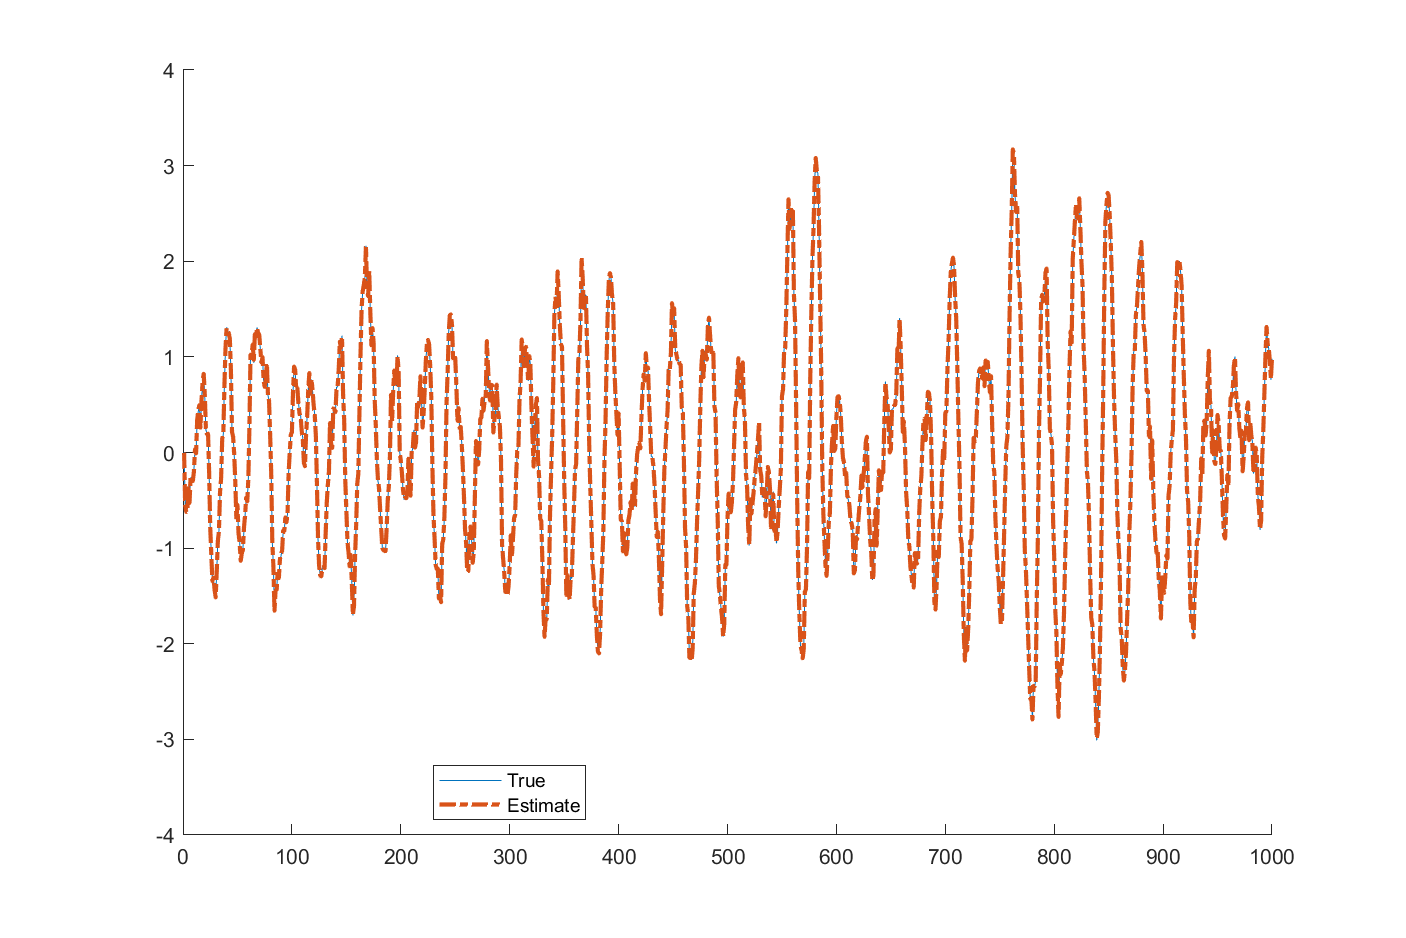
\includegraphics[width=\linewidth]{output_4b.png}
                \caption{Comparison of observer and true states}
                \label{fig:7}
            \end{figure}
        \end{subparts}

        \clearpage
        \part{Repeat the estimation process about 10 times using new values for the new vector each time. Compute the mean and standard deviation of your parameter estimates. Compare the computed values of the parameter statistics with those predicted by the theory based on the known value of the noise statistics.}

        \solution{%
            Running the simulation 10 times with new noise each time allows to take the expectation of our parameters and find the standard deviation of them over 10 runs.
            \begin{equation}
                \begin{split}
                    \overline{x_0} & = 0.2465 \\
                    \overline{x_1} & = -0.1571 \\
                    \overline{x_2} & = 0.4956 \\
                    \overline{x_3} & = -0.3025 \\
                \end{split}
                \label{eq:19}
            \end{equation}
            \begin{equation}
                \begin{split}
                    \sigma_{x_0} & = 0.0235\\
                    \sigma_{x_1} & = 0.0223\\
                    \sigma_{x_2} & = 0.0366\\
                    \sigma_{x_3} & = 0.0218\\
                \end{split}
                \label{eq:20}
            \end{equation}
            Comparing these values to our true parameters and standard deviations we can see that parameters are decently accurate but the standard deviations are not. This is probably due to only running 10 simulations. Running more simulations would lead to a more accurate standard deviation characterization.
            \begin{table}[h!]
                \centering
                \begin{tabular}{|c|c|c|c|}
                    \hline
                    Parameter  & Estimated Value & Theoretical Value & Percent Error (\%) \\
                    \hline
                    $x_0$      & $0.2465$        & $0.25$            & $1.04$             \\
                    $x_1$      & $-0.1571$       & $0.2$             & $172.04$           \\
                    $x_2$      & $0.4956$        & $1.9$             & $72.81$            \\
                    $x_3$      & $-0.3025$       & $0.95$            & $130.54$           \\
                    \hline
                    $\sigma_0$ & $0.0235$        & $9\times10^{-6}$  & $2.432\times10^5$  \\
                    $\sigma_1$ & $0.0223$        & $2\times10^{-5}$  & $9.1586\times10^5$ \\
                    $\sigma_2$ & $0.0366$        & $3\times10^{-4}$  & $7.8579\times10^4$ \\
                    $\sigma_3$ & $0.0218$        & $3\times10^{-4}$  & $6.4201\times10^4$ \\
                    \hline
                \end{tabular}
            \end{table}
        }
        \clearpage
        \part{Now use the sigma between $0.1$ and $1.0$ and repeat parts (b) and (c)}

        \solution{%
            \begin{figure}[!h]
                \centering
                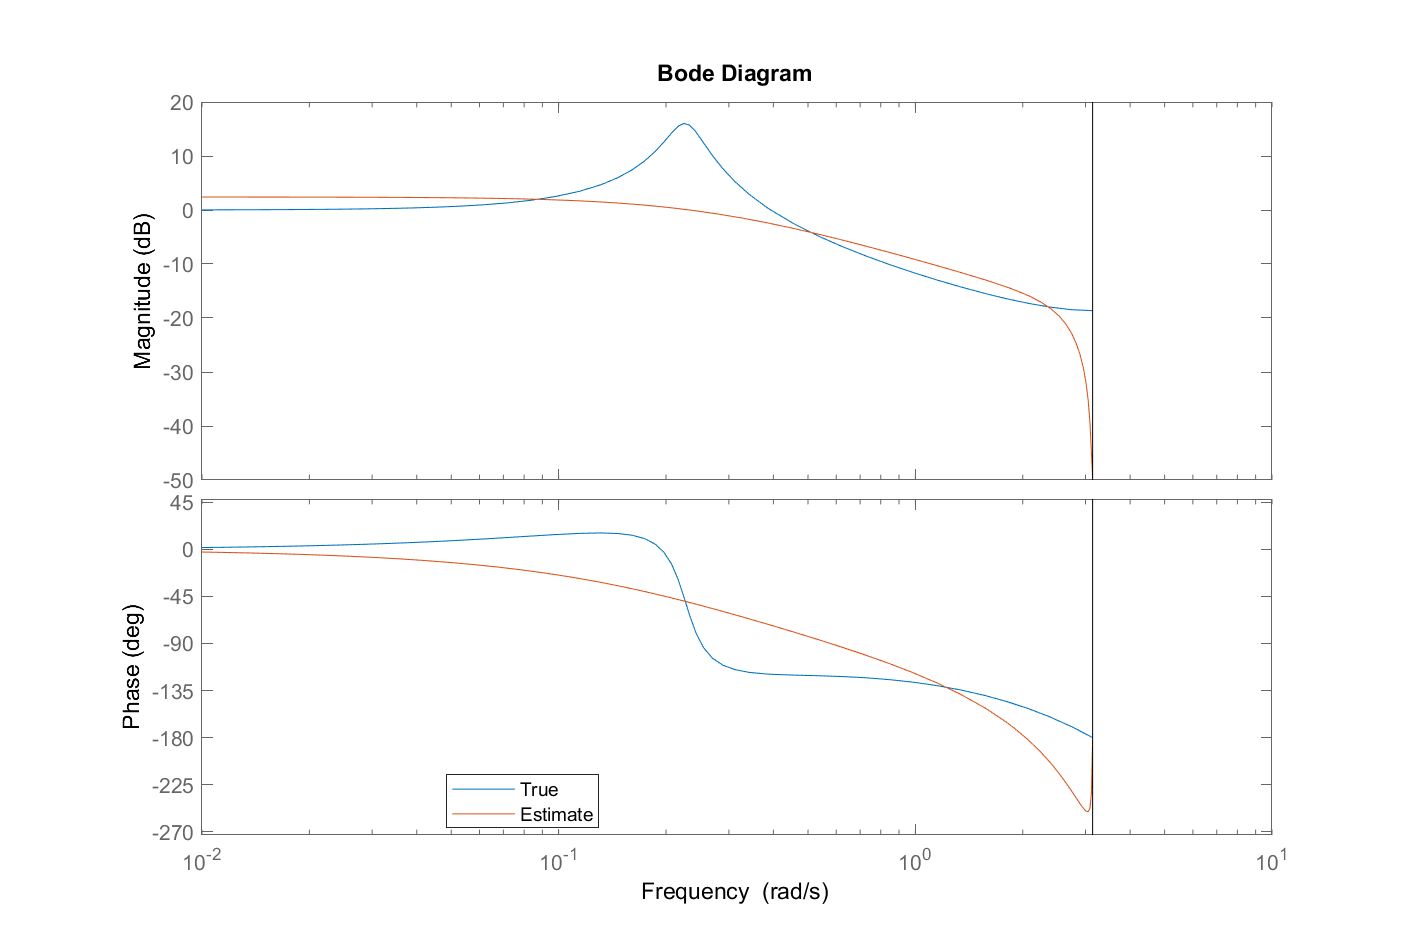
\includegraphics[width=0.75\linewidth]{bode_4d.png}
                \caption{Bode comparison of estimated and true states from Equation \eqref{eq:15}}
                \label{fig:8}
            \end{figure}

            \begin{figure}[!h]
                \centering
                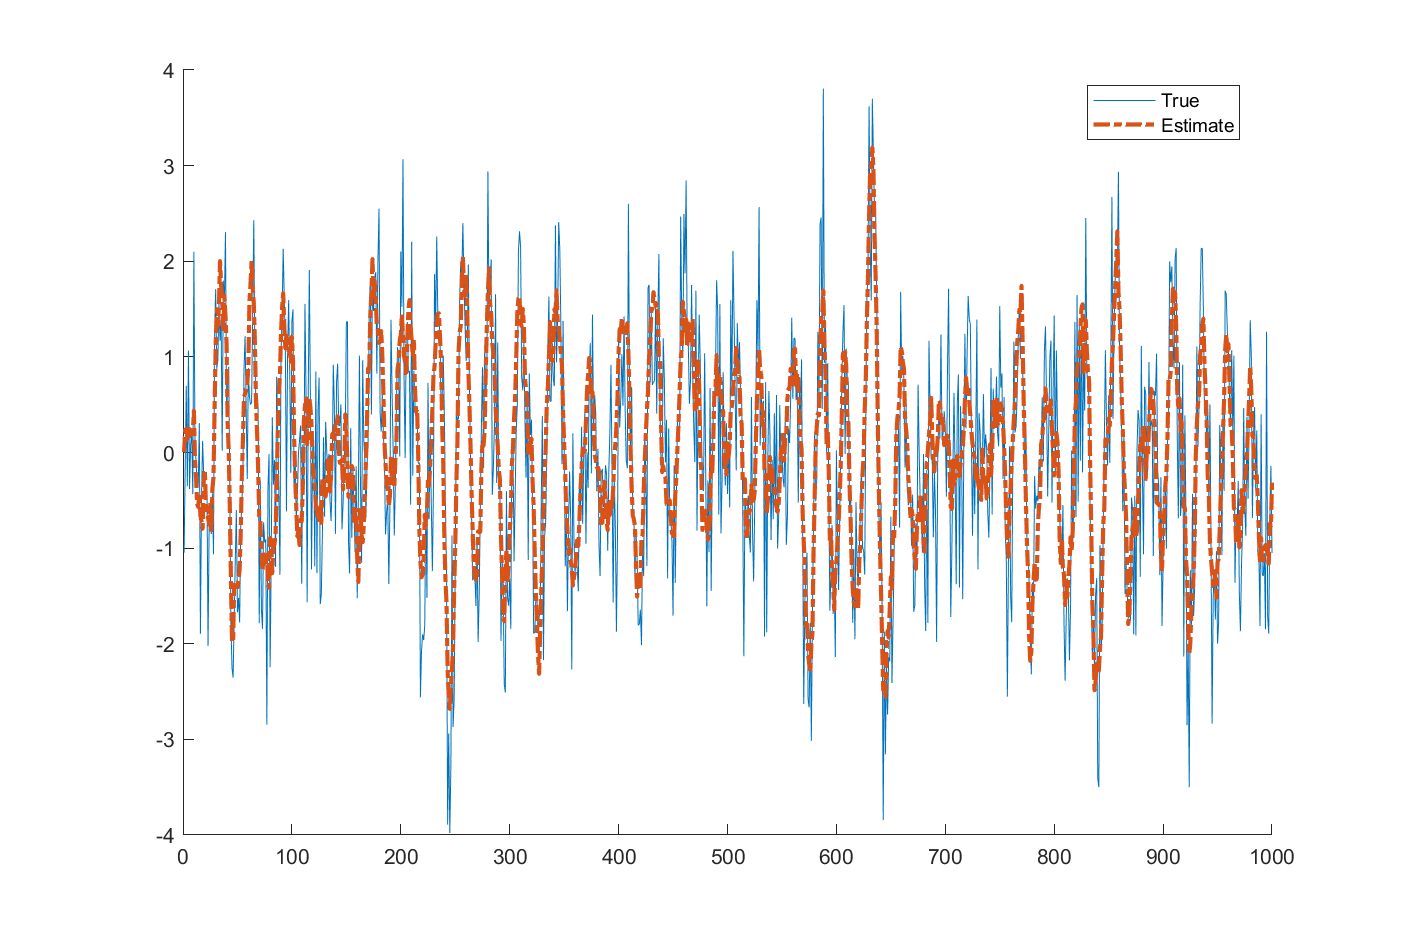
\includegraphics[width=0.75\linewidth]{output_4d.png}
                \caption{Comparison of observer and true states}
                \label{fig:9}
            \end{figure}
            \clearpage
            \begin{table}[h!]
                \centering
                \begin{tabular}{|c|c|c|c|}
                    \hline
                    Parameter  & Estimated Value & Theoretical Value & Percent Error (\%) \\
                    \hline
                    $x_0$      & $0.2427$        & $0.25$            & $2.90$             \\
                    $x_1$      & $-0.1562$       & $0.2$             & $178.09$           \\
                    $x_2$      & $0.5002$        & $1.9$             & $73.68$            \\
                    $x_3$      & $-0.2992$       & $0.95$            & $131.49$           \\
                    \hline
                    $\sigma_0$ & $0.0212$        & $9\times10^{-6}$  & $2.356\times10^5$  \\
                    $\sigma_1$ & $0.022$         & $2\times10^{-5}$  & $9.1586\times10^5$ \\
                    $\sigma_2$ & $0.0523$        & $3\times10^{-4}$  & $1.734\times10^4$  \\
                    $\sigma_3$ & $0.0338$        & $3\times10^{-4}$  & $1.12\times10^4$   \\
                    \hline
                \end{tabular}
            \end{table}
        }
        \part{What can you conclude about using least squares for sys id with large amounts of noise.}

        \solution{%
            Using least squares alone to estimate system states is not a viable option. With a hefty amount of noise, the estimation falls apart and calculates the states including the noise instead of trying to filter it out.
        }
    \end{parts}
    \clearpage
    \question{Justification of white noise for certain problems. Consider two problems:}
    \begin{itemize}
        \item[i.]{Simple first order low-pass filter with bandlimited white noise as the input:
        $y = G(s)\omega$, so that $S_y(j\omega) = \left\vert G(j\omega) \right\vert^2S_{\omega}(j\omega)$, and the noise has the PSD
        \[S_1(\omega) =
            \begin{Bmatrix}
                A & \vert \omega \vert \leq \omega_c \\
                0 & \vert \omega \vert > \omega_c    \\
            \end{Bmatrix} \]
        \[G(s) = \frac{1}{T_{\omega}s + 1} \]
        }
        \item[ii.]{The same low pass system, but with pure white noise as the input.
                    \[S_2(\omega) = A\;\forall\;\omega   \]
                    \[G(s) = \frac{1}{T_{\omega}s + 1} \]
              }
    \end{itemize}
    The first case seems quite plausible, the second case has an input with infinite variance and so is not physically realizable. However, the white noise assumption simplifies the system analysis significantly, so it is important to see if the assumption is justified. We test this with our two examples above:
    \begin{parts}
        \part{Sketch the noise PSD and $\vert G(j\omega)\vert$ for a reasonable value of $T_\omega$ and $\omega)c$ to compare the two cases.}

        \solution{}

        \part{Determine the $S_y(j\omega)$ for the two cases. Sketch these too.}

        \solution{}

        \part{Determine $E[y^2]$ for the two cases.}

        \solution{}

        \part{Use these results to justify the following statement:
            If the input spectrum is flat considerably beyond the system bandwidth, there is little error introduced by assuming that the input spectrum is flat out to infinity.
        }

        \solution{}

    \end{parts}

\end{questions}
\end{document}